\documentclass[11pt]{article}

% Language setting
\usepackage[turkish]{babel}
\usepackage{pythonhighlight}

\usepackage[a4paper,top=2cm,bottom=2cm,left=2cm,right=2cm,marginparwidth=2cm]{geometry}

% Useful packages
\usepackage{amsmath}
\usepackage{graphicx}
\usepackage[colorlinks=true, allcolors=blue]{hyperref}
\usepackage{verbatim}
\usepackage{fancyhdr} % for header and footer
\usepackage{titlesec}
\usepackage{parskip}

\setlength{\parindent}{0pt}

\titleformat{\subsection}[runin]{\bfseries}{\thesubsection}{1em}{}

\pagestyle{fancy} % activate the custom header/footer

% define the header/footer contents
\lhead{\small{23BLM-4014 Yapay Sinir Ağları Ara Sınav Soru ve Cevap Kağıdı}}
\rhead{\small{Dr. Ulya Bayram}}
\lfoot{}
\rfoot{}

% remove header/footer on first page
\fancypagestyle{firstpage}{
  \lhead{}
  \rhead{}
  \lfoot{}
  \rfoot{\thepage}
}
 

\title{Çanakkale Onsekiz Mart Üniversitesi, Mühendislik Fakültesi, Bilgisayar Mühendisliği Akademik Dönem 2022-2023\\
Ders: BLM-4014 Yapay Sinir Ağları/Bahar Dönemi\\ 
ARA SINAV SORU VE CEVAP KAĞIDI\\
Dersi Veren Öğretim Elemanı: Dr. Öğretim Üyesi Ulya Bayram}
\author{%
\begin{minipage}{\textwidth}
\raggedright
Öğrenci Adı Soyadı:Hüdanur ENGİN\\ % Adınızı soyadınızı ve öğrenci numaranızı noktaların yerine yazın
Öğrenci No: 180401051
\end{minipage}%
}

\date{14 Nisan 2023}

\begin{document}
\maketitle

\vspace{-.5in}
\section*{Açıklamalar:}
\begin{itemize}
    \item Vizeyi çözüp, üzerinde aynı sorular, sizin cevaplar ve sonuçlar olan versiyonunu bu formatta PDF olarak, Teams üzerinden açtığım assignment kısmına yüklemeniz gerekiyor. Bu bahsi geçen PDF'i oluşturmak için LaTeX kullandıysanız, tex dosyasının da yer aldığı Github linkini de ödevin en başına (aşağı url olarak) eklerseniz bonus 5 Puan! (Tavsiye: Overleaf)
    \item Çözümlerde ya da çözümlerin kontrolünü yapmada internetten faydalanmak, ChatGPT gibi servisleri kullanmak serbest. Fakat, herkesin çözümü kendi emeğinden oluşmak zorunda. Çözümlerinizi, cevaplarınızı aşağıda belirttiğim tarih ve saate kadar kimseyle paylaşmayınız. 
    \item Kopyayı önlemek için Github repository'lerinizin hiçbirini \textbf{14 Nisan 2023, saat 15:00'a kadar halka açık (public) yapmayınız!} (Assignment son yükleme saati 13:00 ama internet bağlantısı sorunları olabilir diye en fazla ekstra 2 saat daha vaktiniz var. \textbf{Fakat 13:00 - 15:00 arası yüklemelerden -5 puan!}
    \item Ek puan almak için sağlayacağınız tüm Github repository'lerini \textbf{en geç 15 Nisan 2023 15:00'da halka açık (public) yapmış olun linklerden puan alabilmek için!}
    \item \textbf{14 Nisan 2023, saat 15:00'dan sonra gönderilen vizeler değerlendirilmeye alınmayacak, vize notu olarak 0 (sıfır) verilecektir!} Son anda internet bağlantısı gibi sebeplerden sıfır almayı önlemek için assignment kısmından ara ara çözümlerinizi yükleyebilirsiniz yedekleme için. Verilen son tarih/saatte (14 Nisan 2023, saat 15:00) sistemdeki en son yüklü PDF geçerli olacak.
    \item Çözümlerin ve kodların size ait ve özgün olup olmadığını kontrol eden bir algoritma kullanılacaktır. Kopya çektiği belirlenen vizeler otomatikman 0 (sıfır) alacaktır. Bu nedenle çözümlerinizi ve kodlarınızı yukarıda sağladığım gün ve saatlere kadar kimseyle paylaşmayınız.
    \item Bu vizeden alınabilecek en yüksek not 100'dür. Toplam aldığınız puan 100'ü geçerse, aldığınız not 100'e sabitlenecektir.
    \item LaTeX kullanarak PDF oluşturanlar öz geçmişlerine LaTeX bildiklerini de eklemeyi unutmasınlar :)
    \item Bu vizedeki soruların çözümleri ve tex dosyası için istediğiniz kadar sayıda Github repository'si oluşturabilirsiniz. Sadece yukarıda belirttiğim tarihlerde (14 Nisan 2023 saat 15:00 ile 15 Nisan 2023 saat 15:00 arasında) public yapmayı/halka açmayı ve Github profilinizi de öz geçmişinize eklemeyi unutmayın :)
    \item Bilgisayarınıza hiçbir program kurmadan, Overleaf, Google Colab, Kaggle gibi ortamlar üzerinden bu vizeyi tamamlamanız mümkün. İyi çalışmalar!!
\end{itemize}

(Ekstra 5 puan) \url{https://github.com/hudanurengin/artificial-neural-network-latex-report}

\newpage
\section{(Toplam 10 Puan) Hopfield Networks:}

\subsection{(2 Puan)} \textbf{ChatGPT’ye size Hopfield Network’ler ile ilgili detaylı bilgi vermesini isteyin. Sorduğunuz soruyu, ChatGPT'nin çıkartığı cevabı aşağı koyun. Bu cevapta anlamadığınız terimleri de ChatGPT’ye sorup, sorduğunuz soruları ve ChatGPT’nin verdiği cevapları da sırayla aşağı koyun.}

Hopfield Network’ler ile ilgili detaylı bilgi verir misin?

Hopfield ağları, otomatik olarak öğrenen ve hafızaya alan bir yapay sinir ağıdır. Bu ağlar, sınıflandırma, tanıma, çıkarım ve optimizasyon gibi farklı uygulamalar için kullanılabilir.

Hopfield ağları, bir dizi bağlantılı nöronu içerir. Her nöron, diğer tüm nöronlarla bağlantılıdır ve bir nöronun çıkışı, diğer nöronların girdisi olarak kullanılabilir. Ağın her nöronu iki durum alabilir: "aktif" veya "pasif". Ayrıca, her nöronun bir "eşik" değeri vardır, bu değer nöronun aktivasyonunun ne zaman gerçekleşeceğini belirler.

Hopfield ağları, iki temel modda çalışır: öğrenme ve hatırlama. Öğrenme modunda, ağa öğrenme için verilen veriler öğretilir. Bu veriler, ağın bağlantıları arasındaki ağırlıkları değiştirmek için kullanılır. Hatırlama modunda, ağa önceden öğrenilen bilgileri sunulur ve ağ, bu bilgileri kullanarak girdilere en yakın değerleri hatırlar.

Hopfield ağları, gürültülü girdilere dayanıklıdır ve hatırlama işlevi, ağın öğrenme sırasında öğrendiği örüntülerin benzerlerini tanımlayabilmesini sağlar. Ayrıca, Hopfield ağları, yüksek boyutlu veri kümeleri için kullanılabilen bir çözüm sunar.

Hopfield ağları, bellek ve optimizasyon problemlerinin çözümünde kullanılır. Örneğin, Hopfield ağları, en kısa yol sorunları, sıralama sorunları, hatalı veri düzeltme gibi çeşitli problemlerin çözümünde kullanılabilir.

Sonuç olarak, Hopfield ağları, öğrenme, hatırlama, bellek ve optimizasyon problemlerinin çözümünde kullanılan etkili bir yapay sinir ağıdır. 

\subsection{(8 Puan)} \textbf{ChatGPT’nin açıklamalarından ne anladığınızı buraya kendi kelimelerinizle özetleyin. Örneğin ``Hopfield Network nedir? Ne işe yarar? Neden bilmemiz gerekir bunu? Gerçek hayatta kullanılıyor mu?'' gibi. Anlamadığınız kısımlar varsa ve ChatGPT’nin açıklamaları yeterli gelmezse internet dahil farklı kaynaklardan araştırıp, bilgilerin doğruluğunu sorgulamakta serbestsiniz. Konuyu doğru anlayıp anlamamanız puana etki edecektir. Kullandığınız kaynakları da belirtin!}

Hopfield Network öğrenen ve hafızalı bir yapay sinir ağıdır. Sınıflandırma ve optimizasyon gibi konularda kullanılabildiğini öğrendim. 

Örneğin bir ticari firma, depolama alanını optimize etmek isteyebilir. Hopfield ağı, depolama alanını optimize etmek için hangi ürünlerin nerede saklanacağına karar vermek için kullanılabiliyor. Girdiğimiz bir şirkette böyle bir ihtiyaç karşısında çok rahat bir şekilde çözüm üretebilir ve kullanabiliriz.

Hafızalı bir yapay sinir ağı olduğu için bir çok kişinin isim,yüz veya diğer bilgileri hatırlaması gerektiğinde  verimli olarak kullanılabilir.

Hafızalı olması gürültüleri verileri eğitirken avantaj sağlayıp hafızası sayesinde öğrendiği örüntülerle yeni verileri karşılaştırıp benzerliklerini kolayca tespit eder.

Özet olarak,Hopfield ağları, bellek ve optimizasyon problemlerini çözmek için kullanılan bir tür yapay sinir ağıdır. Yüksek doğruluk oranlarına sahiptirler ve birçok alanda kullanılabilirler.

\section{(Toplam 10 Puan) Boltzman Machine:}

\subsection{(2 Puan)} \textbf{ChatGPT’ye size Boltzman Machine ilgili detaylı bilgi vermesini isteyin. Sorduğunuz soruyu, ChatGPT'nin çıkartığı cevabı aşağı koyun. Bu cevapta anlamadığınız terimleri de ChatGPT’ye sorup, sorduğunuz soruları ve ChatGPT’nin verdiği cevapları da sırayla aşağı koyun.}

Boltzman Machine ilgili detaylı bilgi verir misin?

Boltzmann makineleri, yapay sinir ağlarının bir alt türüdür ve olasılık temelli bir modelleme yaklaşımı kullanır. Bu makineler, öğrenme, örüntü tanıma ve veri sıkıştırma gibi uygulamalarda kullanılabilir.

Bir Boltzmann makinesi, birbirine bağlı bir dizi "gizli" ve "gözlemci" nöronlardan oluşur. Gizli nöronlar, gözlemcilerin göremediği içsel değişkenleri temsil ederken, gözlemci nöronlar, verilerin girdi olarak alındığı ve sonuçların üretildiği yerdir.

Bir Boltzmann makinesi, bir enerji fonksiyonu kullanarak çalışır. Bu fonksiyon, ağın tüm nöronları arasındaki bağlantıları içerir ve ağın mevcut durumuna bağlı olarak hesaplanır. Ağ, enerji fonksiyonunu minimize etmek için çalışır ve bunu yaparken, sistemin en olası durumlarından birini bulur.

Bir Boltzmann makinesi, iki modda çalışır: öğrenme ve tahmin. Öğrenme modunda, ağa öğrenme için veriler öğretilir. Bu veriler, ağın bağlantıları arasındaki ağırlıkları değiştirmek için kullanılır. Tahmin modunda, ağa bir girdi verilir ve ağ, girdiye en uygun çıktıyı üretir.

Boltzmann makineleri, özellikle belirsizlik, eksik bilgi ve gürültülü verilerle çalıştıklarında etkilidir. Bu makineler, özellikle verilerin yüksek boyutlara sahip olduğu ve özellikle doğrusal olmayan ilişkilerin bulunduğu uygulamalarda başarılıdır.

Bir Boltzmann makinesi, diğer sinir ağlarına kıyasla daha yavaş öğrenme ve hesaplama işlemleri gerektirir. Ancak, Boltzmann makineleri, özellikle karmaşık problemler için kullanıldığında, etkili sonuçlar verebilir.

Sonuç olarak, Boltzmann makineleri, öğrenme, örüntü tanıma ve veri sıkıştırma gibi uygulamalarda kullanılan olasılık temelli bir modelleme yaklaşımıdır. Bu makineler, özellikle belirsizlik ve eksik bilgi içeren verilerle çalıştıklarında etkilidir.

\subsection{(8 Puan)} \textbf{ChatGPT’nin açıklamalarından ne anladığınızı buraya kendi kelimelerinizle özetleyin. Örneğin ``Boltzman Machine nedir? Ne işe yarar? Neden bilmemiz gerekir bunu? Gerçek hayatta kullanılıyor mu?'' gibi. Anlamadığınız kısımlar varsa ve ChatGPT’nin açıklamaları yeterli gelmezse internet dahil farklı kaynaklardan araştırıp, bilgilerin doğruluğunu sorgulamakta serbestsiniz. Konuyu doğru anlayıp anlamamanız puana etki edecektir. Kullandığınız kaynakları da belirtin!}

Boltzmann makineleri, 2 tür nörondan oluşuyormuş.Bu durumu daha önce duymamıştım.

Gizli nöronlar, belirli bir problem alanındaki özellikleri temsil etmek için kullanılıyor. Örneğin, bir görüntü işleme uygulamasında, gizli nöronlar, görüntünün özelliklerini (örneğin kenarlar, köşeler, renkler vb.) temsil etmek için kullanılabiliyor.

Görünür nöronlar ise, belirli bir problem alanındaki verileri (örneğin, görüntüler, metinler, sayılar vb.) temsil etmek için kullanılıyor. Görünür nöronlar, bir görüntü işleme uygulamasında, görüntüyü piksellerin bir listesi olarak temsil etmek için kullanılabiliyor.

Bir Boltzmann makinesi, gizli ve görünür nöronlar arasında bağlantılar içeren bir ağdır. Bu bağlantılar, bir enerji fonksiyonu kullanılarak hesaplanır. Bu fonksiyon, ağın belirli bir durumda ne kadar enerjiye sahip olduğunu hesaplar. Boltzmann makineleri, bu enerji fonksiyonunu en aza indirmek için çalışır ve en düşük enerjili duruma doğru evrimleşerek belirli bir sorunun çözümünü buluyorlar.

Boltzmann makineleri, özellikle yapay zeka ve derin öğrenme gibi karmaşık bilgi işleme problemlerinin çözümünde kullanılan bir araç. Bu makineler, özellikle bilgisayar görüşü, doğal dil işleme, robotik ve diğer yapay zeka alanlarındaki uygulamalarda kullanılıyor. 

Boltzmann makineleri, yapay zeka uygulamaları için özellikle önemlidir, çünkü bu makineler, belirli bir problem alanındaki en iyi çözüme ulaşmak için rastgele aramalar yaparak çalışıyorlar. Bu nedenle, Boltzmann makineleri, bir sorunu optimize etmek için en iyi çözüme yaklaşmak için kullanılan meta-sezgisel algoritmaların bir örneğidir.

Boltzmann makinelerinin bir diğer dikkat çekici yönü, işlemcilerin artan paralelleştirilmesi sayesinde büyük veri setlerinin işlenmesinde kullanılabilir olmaları. Bu sayede, özellikle görüntü işleme gibi alanlarda çok yüksek boyutlu verilerle çalışmak mümkün hale geliyor.

Günlük hayatta Boltzmann makinelerinin doğrudan kullanımı yokmuş, ancak bu makinelerin temel prensipleri, yapay zeka teknolojilerinin geliştirilmesinde ve kullanımında önemli bir rol oynuyor.

Bir bilgisayar mühendisi için Boltzmann makinelerini bilmek, yapay zeka alanında çalışırken ihtiyaç duyulacak temel bilgilerden biriymiş. Yapay zeka uygulamalarında, özellikle derin öğrenme ve benzeri teknolojilerde, Boltzmann makinelerinin temel prensipleri önemli bir yer tutuyor ve bu prensiplerin anlaşılması, uygulamaların daha etkili bir şekilde geliştirilmesine yardımcı olabilyor.


\section{(Toplam 10 Puan) Markov Assumption ve Markov Chain:}

\subsection{(2 Puan)} \textbf{ChatGPT’ye size Markov assumption ve Markov Chain ilgili detaylı bilgi vermesini isteyin. Sorduğunuz soruyu, ChatGPT'nin çıkartığı cevabı aşağı koyun. Bu cevapta anlamadığınız terimleri de ChatGPT’ye sorup, sorduğunuz soruları ve ChatGPT’nin verdiği cevapları da sırayla aşağı koyun.}

Markov assumption ile ilgili detaylı bilgi verir misin?

Markov varsayımı, bir sistemin gelecekteki durumunu, yalnızca mevcut durumuna bağlı olarak belirleyebileceğimizi varsayar. Bu varsayım, bir dizi olayın ardışık olarak gerçekleştiği durumlarda, sonraki olayların sadece mevcut durumla ilgili olduğu durumlarda uygulanabilir.

Markov varsayımı, daha önceki olayların gelecekteki olayları etkilemediği ve yalnızca mevcut durumun gelecekteki olayları belirlediği anlamına gelir. Bu varsayım, özellikle zaman serileri analizi ve makine öğrenmesi gibi birçok uygulamada yaygın olarak kullanılır.

Markov varsayımı, birinci ve ikinci dereceden Markov modelleri olarak da adlandırılan iki temel modele ayrılır. Birinci dereceden Markov modeli, sadece mevcut duruma bağlı olan bir sonraki durumu modellemek için kullanılır. İkinci dereceden Markov modeli, mevcut duruma ve önceki duruma bağlı olarak bir sonraki durumu modellemek için kullanılır.

Markov varsayımı, birçok algoritmada kullanılır. Örneğin, Markov zincirleri, bir sistemin durumunu zamana göre modellemek için kullanılan bir algoritmadır. Markov rastgele alanı, belirli bir durumun olasılığına dayalı olarak rastgele bir sonraki durum seçmek için kullanılır.

Markov varsayımı, bir sistemdeki değişkenlerin birbirine bağımlılıklarını azalttığı için birçok uygulamada etkilidir. Ancak, bazı durumlarda bu varsayım geçersiz olabilir. Örneğin, finansal piyasalarda fiyat değişkenleri birbirine bağımlı olduğundan, Markov varsayımı bu durumlarda geçerli olmayabilir.

Sonuç olarak, Markov varsayımı, bir sistemin gelecekteki durumunu yalnızca mevcut duruma bağlı olarak belirleyebileceğimizi varsayar. Bu varsayım, birçok uygulamada kullanılır ve bir sistemdeki değişkenlerin birbirine bağımlılıklarını azaltır. Ancak, bazı durumlarda geçerli olmayabilir.

Markov Chain  ile ilgili detaylı bilgi verir misin?

Markov zinciri, bir sistemin durumunu zamana göre modelleyen matematiksel bir yapıdır. Bir sistemdeki durumlar, zamanın ilerlemesiyle birbirini takip eder ve her durumun olasılığı, yalnızca önceki duruma bağlıdır. Bu nedenle, Markov zincirleri, birinci dereceden Markov modelleri olarak da adlandırılır.

Markov zincirleri, matematiksel olarak bir durum kümesi ve her durumun bir sonraki durum için olasılıklarını gösteren bir geçiş matrisi ile tanımlanır. Geçiş matrisinde, her satır bir durumu ve her sütun bir sonraki durumu temsil eder. Her hücredeki değer, bir durumdan diğerine geçme olasılığını gösterir.

Bir Markov zincirinin belirli özellikleri vardır. İlk olarak, herhangi bir zaman dilimindeki durumlar, tüm geçmiş durumlarını etkilemez, yalnızca son durumdan etkilenirler. İkinci olarak, zincir, durumların zamanla değiştiği ve belirli bir zaman dilimi boyunca durumun aynı kalabileceği birçok durumdan oluşur. Üçüncü olarak, zincir, durumlar arasında geçişlerin sürekli olduğu bir yapıya sahiptir.

Markov zincirleri, birçok uygulama alanında kullanılır. Örneğin, doğal dil işlemede bir kelimenin bir sonraki kelime olarak ne olabileceğini tahmin etmek için kullanılırlar. Ayrıca, ekonomi, finans, fizik, biyoloji, mühendislik ve diğer birçok alanda kullanılırlar.

Markov zincirleri, birçok algoritma ve teknikle birlikte kullanılabilir. Örneğin, çarpım zinciri algoritması, bir zincirin gelecekteki durumlarını tahmin etmek için kullanılır. Monte Carlo yöntemleri, bir zincirdeki olasılıkları tahmin etmek için kullanılır. Ayrıca, bir zincirin dengeli dağılımı ve sınır davranışı gibi özellikleri de çeşitli uygulamalarda önemlidir.

Sonuç olarak, Markov zincirleri, bir sistemin durumunu zamana göre modelleyen matematiksel bir yapıdır. Her durumun olasılığı, yalnızca önceki duruma bağlıdır ve birinci dereceden Markov modelleri olarak adlandırılır. Birçok uygulama alanında kullanılırlar ve birçok algoritma ve teknikle birlikte kullanılabilirler.

\subsection{(8 Puan)} \textbf{ChatGPT’nin açıklamalarından ne anladığınızı buraya kendi kelimelerinizle özetleyin. Örneğin ``Markov assumption ve Markov Chain nedir? Ne işe yarar? Neden bilmemiz gerekir bunu? Gerçek hayatta kullanılıyor mu?'' gibi. Anlamadığınız kısımlar varsa ve ChatGPT’nin açıklamaları yeterli gelmezse internet dahil farklı kaynaklardan araştırıp, bilgilerin doğruluğunu sorgulamakta serbestsiniz. Konuyu doğru anlayıp anlamamanız puana etki edecektir. Kullandığınız kaynakları da belirtin!}

Markov varsayımı

Markov varsayımı, belirli bir sistemin gelecekteki durumu, yalnızca o sistemin şimdiki durumuna bağlı ve geçmiş durumlarla ilgilenmiyor. Bu varsayım, birçok modellemede kullanılıyor ve Markov zinciri, Markov karar süreci, Markov rastgele alanı ve benzeri kavramların temelini oluşturuyor.

Markov varsayımı, özellikle doğal dil işleme, yapay zeka, sinyal işleme ve finansal piyasalar gibi alanlarda aktif olarak kullanılmakta Örneğin, bir doğal dil işleme modelinde, bir kelimenin olası bir sonraki kelimeye göre tahmin edilmesi için Markov varsayımı kullanılabilir.

Bir bilgisayar mühendisi olarak Markov varsayımını bilmek, makine öğrenimi, yapay zeka ve optimizasyon gibi alanlarda modelleme yaparken yardımcı olabilir. Ayrıca, finansal piyasaların modellemesi gibi çeşitli uygulamalarda da kullanılabilir.

En basit şekilde ifade etmek gerekirse, Markov varsayımı, gelecekteki durumların yalnızca mevcut duruma bağlı olduğunu varsayar. Bu varsayım, birçok modellemede kullanılır ve bir sistemdeki önceki durumlarla ilgilenmeden gelecekteki durumların tahmin edilmesine yardımcı olabilir.

Markov Chain

Markov Chain Rule mevcut durum verildiğinde, gelecek durumların geçmiş durumlardan bağımsız olması anlamına gelir. Yani geleceğimiz sadece şu an içinde bulunduğumuz durumdan etkilenir. Geçmişimiz önemsizdir.

Bu modelde, her bir anda sistem belirli bir olasılık dağılımına bağlı olarak kendi durumundan başka bir duruma geçebilir veya aynı durumda kalabilir. Durumda olan değişiklikler geçiş olarak bilinir ve çeşitli durum değişmeleriyle ilişkili olasılıklar da geçiş olasılıkları olarak adlandırılır.

Bir yolda olduğunuzu düşünün yol sadece A,B,C ,D ve E şehirlerinden ve sırayla geçiyor. Eğer şu an C şehrindeysek gelecekte D veya B şehrine gideceğimizi biliriz. Bu kanıya varmak için C şehrine gelmeden önce nerede olduğumuzun bir önemi yok.

Bir bilgisayar mühendisi olarak Markov zincirini bilmek, makine öğrenimi, yapay zeka ve optimizasyon gibi alanlarda modelleme yaparken yardımcı olabilir. Ayrıca, finansal piyasaların modellemesi gibi çeşitli uygulamalarda da kullanılabilir.

En basit şekilde ifade etmek gerekirse, Markov zinciri, rastgele bir sürecin matematiksel bir modelidir ve gelecekteki durumlar, yalnızca mevcut durumlara bağlıdır. Bu model, birçok alanda kullanılır ve bir sistemdeki önceki durumlarla ilgilenmeden gelecekteki durumların tahmin edilmesine yardımcı olabilir.


\section{(Toplam 20 Puan) Feed Forward:}
 
\begin{itemize}
    \item Forward propagation için, input olarak şu X matrisini verin (tensöre çevirmeyi unutmayın):\\
    $X = \begin{bmatrix}
        1 & 2 & 3\\
        4 & 5 & 6
        \end{bmatrix}$
    Satırlar veriler (sample'lar), kolonlar öznitelikler (feature'lar).
    \item Bir adet hidden layer olsun ve içinde tanh aktivasyon fonksiyonu olsun
    \item Hidden layer'da 50 nöron olsun
    \item Bir adet output layer olsun, tek nöronu olsun ve içinde sigmoid aktivasyon fonksiyonu olsun
\end{itemize}

Tanh fonksiyonu:\\
$f(x) = \frac{exp(x) - exp(-x)}{exp(x) + exp(-x)}$
\vspace{.2in}

Sigmoid fonksiyonu:\\
$f(x) = \frac{1}{1 + exp(-x)}$

\vspace{.2in}
 \textbf{Pytorch kütüphanesi ile, ama kütüphanenin hazır aktivasyon fonksiyonlarını kullanmadan, formülünü verdiğim iki aktivasyon fonksiyonunun kodunu ikinci haftada yaptığımız gibi kendiniz yazarak bu yapay sinir ağını oluşturun ve aşağıdaki üç soruya cevap verin.}
 
\subsection{(10 Puan)} \textbf{Yukarıdaki yapay sinir ağını çalıştırmadan önce pytorch için Seed değerini 1 olarak set edin, kodu aşağıdaki kod bloğuna ve altına da sonucu yapıştırın:}

% Latex'de kod koyabilirsiniz python formatında. Aşağıdaki örnekleri silip içine kendi kodunuzu koyun
\begin{python}
import torch

x = torch.tensor([[1, 2, 3], [4, 5, 6]], dtype=torch.float)
x=torch.flatten(x)
x

torch.manual_seed(1)
input_size = 6
hidden_size = 50
hidden_weight= torch.randn(input_size, hidden_size)
hidden_bias = torch.randn(hidden_size)


output_size = 1
output_weight = torch.randn(hidden_size, output_size)
output_bias = torch.randn(output_size)

def sigmoid_activation(x):

  return 1 / (1 + torch.exp(-x))

  def tanh_activation(x):

    return (torch.exp(x) - torch.exp(-x))/(torch.exp(x) + torch.exp(-x))

#hidden layer
hidden_layer = torch.matmul(x, hidden_weight) + hidden_bias
hidden_activation= tanh_activation(hidden_layer)
hidden_activation2= torch.tanh(hidden_layer)

# Output layer
output_layer= torch.matmul(hidden_activation, output_weight) + output_bias
output_activation= sigmoid_activation(output_layer)
output_activation2= torch.sigmoid(output_layer)
output_activation,output_activation2
\end{python}

(tensor([0.0575]), tensor([0.0575]))

\subsection{(5 Puan)} \textbf{Yukarıdaki yapay sinir ağını çalıştırmadan önce Seed değerini öğrenci numaranız olarak değiştirip, kodu aşağıdaki kod bloğuna ve altına da sonucu yapıştırın:}

\begin{python}
import torch
x = torch.tensor([[1, 2, 3], [4, 5, 6]], dtype=torch.float)
x=torch.flatten(x)
x

torch.manual_seed(180401051)

input_size = 6
hidden_size = 50

hidden_weight= torch.randn(input_size, hidden_size)
hidden_bias = torch.randn(hidden_size)

output_size = 1

output_weight = torch.randn(hidden_size, output_size)
output_bias = torch.randn(output_size)

def sigmoid_activation(x):

  return 1 / (1 + torch.exp(-x))

def tanh_activation(x):

    return (torch.exp(x) - torch.exp(-x))/(torch.exp(x) + torch.exp(-x))

#hidden layer
hidden_layer = torch.matmul(x, hidden_weight) + hidden_bias
hidden_activation= tanh_activation(hidden_layer)
hidden_activation2= torch.tanh(hidden_layer)

# Output layer
output_layer= torch.matmul(hidden_activation, output_weight) + output_bias
output_activation= sigmoid_activation(output_layer)
output_activation2= torch.sigmoid(output_layer)

output_activation,output_activation2
\end{python}

(tensor([1.0000]), tensor([1.0000]))

\subsection{(5 Puan)} \textbf{Kodlarınızın ve sonuçlarınızın olduğu jupyter notebook'un Github repository'sindeki linkini aşağıdaki url kısmının içine yapıştırın. İlk sayfada belirttiğim gün ve saate kadar halka açık (public) olmasın:}
% size ait Github olmak zorunda, bu vize için ayrı bir github repository'si açıp notebook'u onun içine koyun. Kendine ait olmayıp da arkadaşının notebook'unun linkini paylaşanlar 0 alacak.

\url{https://github.com/hudanurengin/Feed-Forward}

\section{(Toplam 40 Puan) Multilayer Perceptron (MLP):} 
\textbf{Bu bölümdeki sorularda benim vize ile beraber paylaştığım Prensesi İyileştir (Cure The Princess) Veri Seti parçaları kullanılacak. Hikaye şöyle (soruyu çözmek için hikaye kısmını okumak zorunda değilsiniz):} 

``Bir zamanlar, çok uzaklarda bir ülkede, ağır bir hastalığa yakalanmış bir prenses yaşarmış. Ülkenin kralı ve kraliçesi onu iyileştirmek için ellerinden gelen her şeyi yapmışlar, ancak denedikleri hiçbir çare işe yaramamış.

Yerel bir grup köylü, herhangi bir hastalığı iyileştirmek için gücü olduğu söylenen bir dizi sihirli malzemeden bahsederek kral ve kraliçeye yaklaşmış. Ancak, köylüler kral ile kraliçeyi, bu malzemelerin etkilerinin patlayıcı olabileceği ve son zamanlarda yaşanan kuraklıklar nedeniyle bu malzemelerden sadece birkaçının herhangi bir zamanda bulunabileceği konusunda uyarmışlar. Ayrıca, sadece deneyimli bir simyacı bu özelliklere sahip patlayıcı ve az bulunan malzemelerin belirli bir kombinasyonunun prensesi iyileştireceğini belirleyebilecekmiş.

Kral ve kraliçe kızlarını kurtarmak için umutsuzlar, bu yüzden ülkedeki en iyi simyacıyı bulmak için yola çıkmışlar. Dağları tepeleri aşmışlar ve nihayet "Yapay Sinir Ağları Uzmanı" olarak bilinen yeni bir sihirli sanatın ustası olarak ün yapmış bir simyacı bulmuşlar.

Simyacı önce köylülerin iddialarını ve her bir malzemenin alınan miktarlarını, ayrıca iyileşmeye yol açıp açmadığını incelemiş. Simyacı biliyormuş ki bu prensesi iyileştirmek için tek bir şansı varmış ve bunu doğru yapmak zorundaymış. (Original source: \url{https://www.kaggle.com/datasets/unmoved/cure-the-princess})

(Buradan itibaren ChatGPT ve Dr. Ulya Bayram'a ait hikayenin devamı)

Simyacı, büyülü bileşenlerin farklı kombinasyonlarını analiz etmek ve denemek için günler harcamış. Sonunda birkaç denemenin ardından prensesi iyileştirecek çeşitli karışım kombinasyonları bulmuş ve bunları bir veri setinde toplamış. Daha sonra bu veri setini eğitim, validasyon ve test setleri olarak üç parçaya ayırmış ve bunun üzerinde bir yapay sinir ağı eğiterek kendi yöntemi ile prensesi iyileştirme ihtimalini hesaplamış ve ikna olunca kral ve kraliçeye haber vermiş. Heyecanlı ve umutlu olan kral ve kraliçe, simyacının prensese hazırladığı ilacı vermesine izin vermiş ve ilaç işe yaramış ve prenses hastalığından kurtulmuş.

Kral ve kraliçe, kızlarının hayatını kurtardığı için simyacıya krallıkta kalması ve çalışmalarına devam etmesi için büyük bir araştırma bütçesi ve çok sayıda GPU'su olan bir server vermiş. İyileşen prenses de kendisini iyileştiren yöntemleri öğrenmeye merak salıp, krallıktaki üniversitenin bilgisayar mühendisliği bölümüne girmiş ve mezun olur olmaz da simyacının yanında, onun araştırma grubunda çalışmaya başlamış. Uzun yıllar birlikte krallıktaki insanlara, hayvanlara ve doğaya faydalı olacak yazılımlar geliştirmişler, ve simyacı emekli olduğunda prenses hem araştırma grubunun hem de krallığın lideri olarak hayatına devam etmiş.

Prenses, kendisini iyileştiren veri setini de, gelecekte onların izinden gidecek bilgisayar mühendisi prensler ve prensesler başkalarına faydalı olabilecek yapay sinir ağları oluşturmayı öğrensinler diye halka açmış ve sınavlarda kullanılmasını salık vermiş.''

\textbf{İki hidden layer'lı bir Multilayer Perceptron (MLP) oluşturun beşinci ve altıncı haftalarda yaptığımız gibi. Hazır aktivasyon fonksiyonlarını kullanmak serbest. İlk hidden layer'da 100, ikinci hidden layer'da 50 nöron olsun. Hidden layer'larda ReLU, output layer'da sigmoid aktivasyonu olsun.}

\textbf{Output layer'da kaç nöron olacağını veri setinden bakıp bulacaksınız. Elbette bu veriye uygun Cross Entropy loss yöntemini uygulayacaksınız. Optimizasyon için Stochastic Gradient Descent yeterli. Epoch sayınızı ve learning rate'i validasyon seti üzerinde denemeler yaparak (loss'lara overfit var mı diye bakarak) kendiniz belirleyeceksiniz. Batch size'ı 16 seçebilirsiniz.}

\subsection{(10 Puan)} \textbf{Bu MLP'nin pytorch ile yazılmış class'ının kodunu aşağı kod bloğuna yapıştırın:}

\begin{python}
class MLP(nn.Module):
    def __init__(self, input_size, hidden_size1, hidden_size2, output_size):
        super(MLP, self).__init__()
        self.fc1 = nn.Linear(input_size, hidden_size1)
        self.relu1 = nn.ReLU()
        self.fc2 = nn.Linear(hidden_size1, hidden_size2)
        self.relu2 = nn.ReLU()
        self.fc3 = nn.Linear(hidden_size2, output_size)
        self.sigmoid = nn.Sigmoid()
        
    def forward(self, x):
        out = self.fc1(x)
        out = self.relu1(out)
        out = self.fc2(out)
        out = self.relu2(out)
        out = self.fc3(out)
        out = self.sigmoid(out)
        return out
\end{python}

\subsection{(10 Puan)} \textbf{SEED=öğrenci numaranız set ettikten sonra altıncı haftada yazdığımız gibi training batch'lerinden eğitim loss'ları, validation batch'lerinden validasyon loss değerlerini hesaplayan kodu aşağıdaki kod bloğuna yapıştırın ve çıkan figürü de alta ekleyin.}

\begin{python}
batch_size = 32
input_size = 13
hidden_size1 = 100
hidden_size2 = 50
output_size = 1
learning_rate = 0.001
epochs = 100

model = MLP(input_size, hidden_size1, hidden_size2, output_size)
criterion = nn.BCELoss()
optimizer = optim.SGD(model.parameters(), lr=learning_rate)

train_losses = []
val_losses = []
best_model = None
best_val_loss= float('inf')
patience_counter = 0
for epoch in range(epochs):
        # Training
    model.train()
    train_loss = 0.0
    for i, (inputs, labels) in enumerate(train_dataloader):
        optimizer.zero_grad()
        outputs = model(inputs.float())
        loss = criterion(outputs, labels)
        loss.backward()
        optimizer.step()
        train_loss += loss.item()
    train_loss /= len(train_dataloader)
    train_losses.append(train_loss)

        # Validation
    model.eval()
    val_loss = 0.0
    with torch.no_grad():
        for i, (inputs, labels) in enumerate(val_dataloader):
            outputs = model(inputs.float())
            loss = criterion(outputs, labels)
            val_loss += loss.item()
    val_loss /= len(val_dataloader)
    val_losses.append(val_loss)

    if (epoch+1) % 10 == 0:
        print(f"Epoch: {epoch+1}/{epochs}, Train Loss: {train_loss:.4f}, Val Loss: {val_loss:.4f}")


sns.set_style("darkgrid")
plt.plot(train_losses, label="Train Loss")
plt.plot(val_losses, label="Val Loss")
plt.xlabel("Epochs")
plt.ylabel("Loss")
plt.legend()
plt.show()

\end{python}



\begin{figure}[ht!]
    \centering
    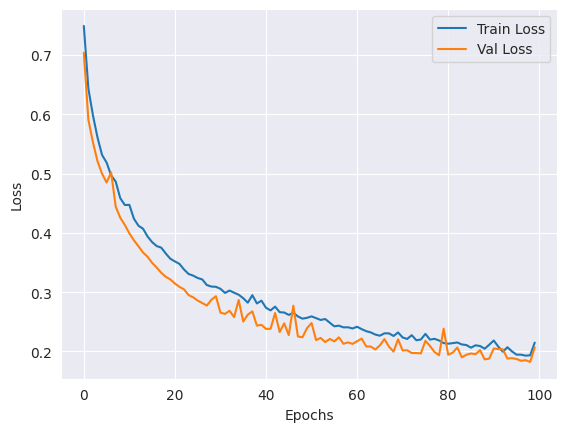
\includegraphics{indir.png}
    \caption{Train-validation görünümleri}
    \label{fig:my_label}
\end{figure}


\subsection{(10 Puan)} \textbf{SEED=öğrenci numaranız set ettikten sonra altıncı haftada ödev olarak verdiğim gibi earlystopping'deki en iyi modeli kullanarak, Prensesi İyileştir test setinden accuracy, F1, precision ve recall değerlerini hesaplayan kodu yazın ve sonucu da aşağı yapıştırın. \%80'den fazla başarı bekliyorum test setinden. Daha düşükse başarı oranınız, nerede hata yaptığınızı bulmaya çalışın. \%90'dan fazla başarı almak mümkün (ben denedim).}

\begin{python}

batch_size = 32
input_size = 13
hidden_size1 = 100
hidden_size2 = 50
output_size = 1
learning_rate = 0.001
epochs = 100
patience=10



model = MLP(input_size, hidden_size1, hidden_size2, output_size)
criterion = nn.BCELoss()
optimizer = optim.SGD(model.parameters(), lr=learning_rate)



train_losses = []
val_losses = []
best_model = None
best_val_loss= float('inf')
patience_counter = 0
for epoch in range(epochs):

        # Training
    model.train()
    train_loss = 0.0
    for i, (inputs, labels) in enumerate(train_dataloader):
        optimizer.zero_grad()
        outputs = model(inputs.float())
        loss = criterion(outputs, labels)
        loss.backward()
        optimizer.step()
        train_loss += loss.item()
    train_loss /= len(train_dataloader)
    train_losses.append(train_loss)



        # Validation
    model.eval()
    val_loss = 0.0
    with torch.no_grad():
        for i, (inputs, labels) in enumerate(val_dataloader):
            outputs = model(inputs.float())
            loss = criterion(outputs, labels)
            val_loss += loss.item()
    val_loss /= len(val_dataloader)
    val_losses.append(val_loss)

    if (epoch+1) % 10 == 0:
        print(f"Epoch: {epoch+1}/{epochs}, Train Loss: {train_loss:.4f}, Val Loss: {val_loss:.4f}")


# Early stopping
    if val_loss < best_val_loss:
        best_val_loss = val_loss
        best_model = model
        patience_counter = 0
    else:
        patience_counter += 1
        if patience_counter >= patience:
            print(f'Early stopping: val_loss has not improved for {patience} epochs')
            break



sns.set_style("darkgrid")
plt.plot(train_losses, label="Train Loss")
plt.plot(val_losses, label="Val Loss")
plt.xlabel("Epochs")
plt.ylabel("Loss")
plt.legend()
plt.show()

#train(model, train_dataloader, val_dataloader, criterion, optimizer, epochs)



tp = 0  # True positives
fp = 0  # False positives
tn = 0  # True negatives
fn = 0  # False negatives
model.eval()
with torch.no_grad():
      for i, (inputs, labels) in enumerate(val_dataloader):
              outputs = model(inputs.float())
              loss = criterion(outputs, labels)
              val_loss += loss.item()
val_loss /= len(val_dataloader)
val_losses.append(val_loss)
predicted_labels = (outputs >= 0.5).float()



# matrisi guncelliyorum
tp += torch.sum(predicted_labels * labels).item()
fp += torch.sum(predicted_labels * (1 - labels)).item()
tn += torch.sum((1 - predicted_labels) * (1 - labels)).item()
fn += torch.sum((1 - predicted_labels) * labels).item()




# accuracy, precision, recall and F1 score
accuracy = (tp + tn) / (tp + tn + fp + fn)
precision = tp / (tp + fp)
recall = tp / (tp + fn)
f1 = 2 * precision * recall / (precision + recall)

print(f'Test Accuracy: {accuracy:.4f}, Test Precision: {precision:.4f}, Test Recall: {recall:.4f}, Test F1: {f1:.4f}')
\end{python}

Test Accuracy: 0.9231, Test Precision: 0.8824, Test Recall: 1.0000, Test F1: 0.9375

\subsection{(5 Puan)} \textbf{Tüm kodların CPU'da çalışması ne kadar sürüyor hesaplayın. Sonra to device yöntemini kullanarak modeli ve verileri GPU'ya atıp kodu bir de böyle çalıştırın ve ne kadar sürdüğünü hesaplayın. Süreleri aşağıdaki tabloya koyun. GPU için Google Colab ya da Kaggle'ı kullanabilirsiniz, iki ortam da her hafta saatlerce GPU hakkı veriyor.}

\begin{table}[ht!]
    \centering
    \caption{Çalışma Süresi Karşılaştırma}
    \begin{tabular}{c|c}
        Ortam & Süre (saniye) \\\hline
        CPU & 27 \\
        GPU & 26\\
    \end{tabular}
    \label{tab:my_table}
\end{table}

\subsection{(3 Puan)} \textbf{Modelin eğitim setine overfit etmesi için elinizden geldiği kadar kodu gereken şekilde değiştirin, validasyon loss'unun açıkça yükselmeye başladığı, training ve validation loss'ları içeren figürü aşağı koyun ve overfit için yaptığınız değişiklikleri aşağı yazın. Overfit, tam bir çanak gibi olmalı ve yükselmeli. Ona göre parametrelerle oynayın.}

batchsize=8
learningrate=0.01 olarak güncelledim.
\begin{figure}
    \centering
    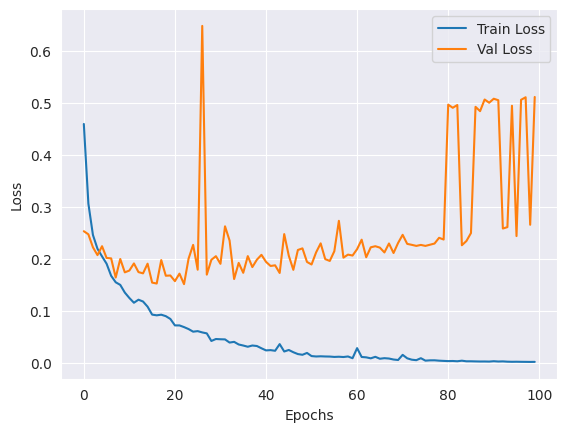
\includegraphics{overfit.png}
    \caption{Overfitting}
    \label{fig:my_label}
\end{figure}

\newpage
\subsection{(2 Puan)} \textbf{Beşinci soruya ait tüm kodların ve cevapların olduğu jupyter notebook'un Github linkini aşağıdaki url'e koyun.}

\url{https://github.com/hudanurengin/Cure-the-princess}

\section{(Toplam 10 Puan)} \textbf{Bir önceki sorudaki Prensesi İyileştir problemindeki yapay sinir ağınıza seçtiğiniz herhangi iki farklı regülarizasyon yöntemi ekleyin ve aşağıdaki soruları cevaplayın.} 

\subsection{(2 puan)} \textbf{Kodlarda regülarizasyon eklediğiniz kısımları aşağı koyun:} 

\begin{python}
kod_buraya = None
if kod_buraya:
    devam_ise_buraya = 0

print(devam_ise_buraya)
\end{python}

\subsection{(2 puan)} \textbf{Test setinden yeni accuracy, F1, precision ve recall değerlerini hesaplayıp aşağı koyun:}

Sonuçlar buraya.

\subsection{(5 puan)} \textbf{Regülarizasyon yöntemi seçimlerinizin sebeplerini ve sonuçlara etkisini yorumlayın:}

Yorumlar buraya.

\subsection{(1 puan)} \textbf{Sonucun github linkini  aşağıya koyun:}

\url{www.benimgithublinkim2.com}

\end{document}